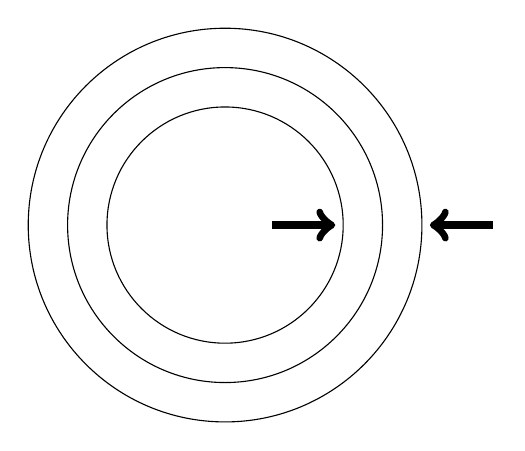
\begin{tikzpicture}
\pgfmathsetmacro{\scale}{2.5}
\pgfmathsetmacro{\parts}{5}
\pgfmathsetmacro{\posOut}{1}
\pgfmathsetmacro{\posMiddle}{0.8}
\pgfmathsetmacro{\posIns}{0.6}

\pgfmathsetmacro{\circles}{\parts*4}
\pgfmathsetmacro{\posOut}{1 * \scale}
\pgfmathsetmacro{\posMiddle}{0.8 * \scale}
\pgfmathsetmacro{\posInside}{0.6 * \scale}
\pgfmathsetmacro{\partAngle}{360 / \circles}
\path (0,0)[draw=black] circle (\posOut);
\path (0,0)[draw=black] circle (\posMiddle);
\path (0,0)[draw=black] circle (\posInside);
\foreach\i in {0,4,...,\circles} {
    \drawStrip{black}{\partAngle}{\i + 0}{\posMiddle}{\posOut}
    \drawStrip{black}{\partAngle}{\i + 1}{\posMiddle}{\posOut}
    \drawStrip{black}{\partAngle}{\i + 1}{\posInside}{\posMiddle}
    \drawStrip{black}{\partAngle}{\i + 2}{\posInside}{\posMiddle}
}
\draw [black,<-,line width=3pt] ({\posInside - 0.1},0) -- +(-0.8,0);
\draw [black,<-,line width=3pt] ({\posOut + 0.1},0) -- +(0.8,0);
\end{tikzpicture}
